In conclusion, the higher the fretting position, the more intonation error there is. The relationship is not a linear one but quite complicated and can be modelled with equation (\ref{eqn39}). By plotting the data and performing the goodness-of-fit test, it reasonably confirms the validity of the equation. \par
By choosing this simplified model, it makes the calculations easier and creates a useful approximation model. However, this doesn't take into account several factors in reality that can affect the intonation. For example, the contact surface of a capo on the string is quite large compared to a human finger; therefore the string might deform more when using the capo, increasing the tension and frequency. Also, normally guitarists don't press down directly on the fret like the capo, but slightly behind. This can depress the string more and lead to higher intonation errors. Another factor is the guitar neck isn't always rigid and straight but sometimes slightly bowed, either from the tension of the strings or from the player's setup, which can also affect the intonation. An assumption I made is the fretting point on the string would have no friction, thus tension will increase evenly throughout the string, but in reality the finger or capo would have a small amount of friction that can affect the result. Another limitation of the model is it only applies to plain unwound steel strings, so it can only be used for the highest 3 strings on an electric guitar, but for the other 3 wound strings we would need a different model.\par

An observation I can make from equation (\ref{eqn39}) is that it is not dependent on the string gauge I use. However, this conflicts with my experience, because when playing I would notice the thicker G string would exhibit more intonation shift than the thinner high E string. To investigate this, I repeat the experiment with my thinner B string and E string, tuning them to their standard frequencies ($B_3: 246.94$Hz and $E_4: 329.63$Hz). The collected and processed data for these are in the Appendix.

\begin{figure}[!htb]
    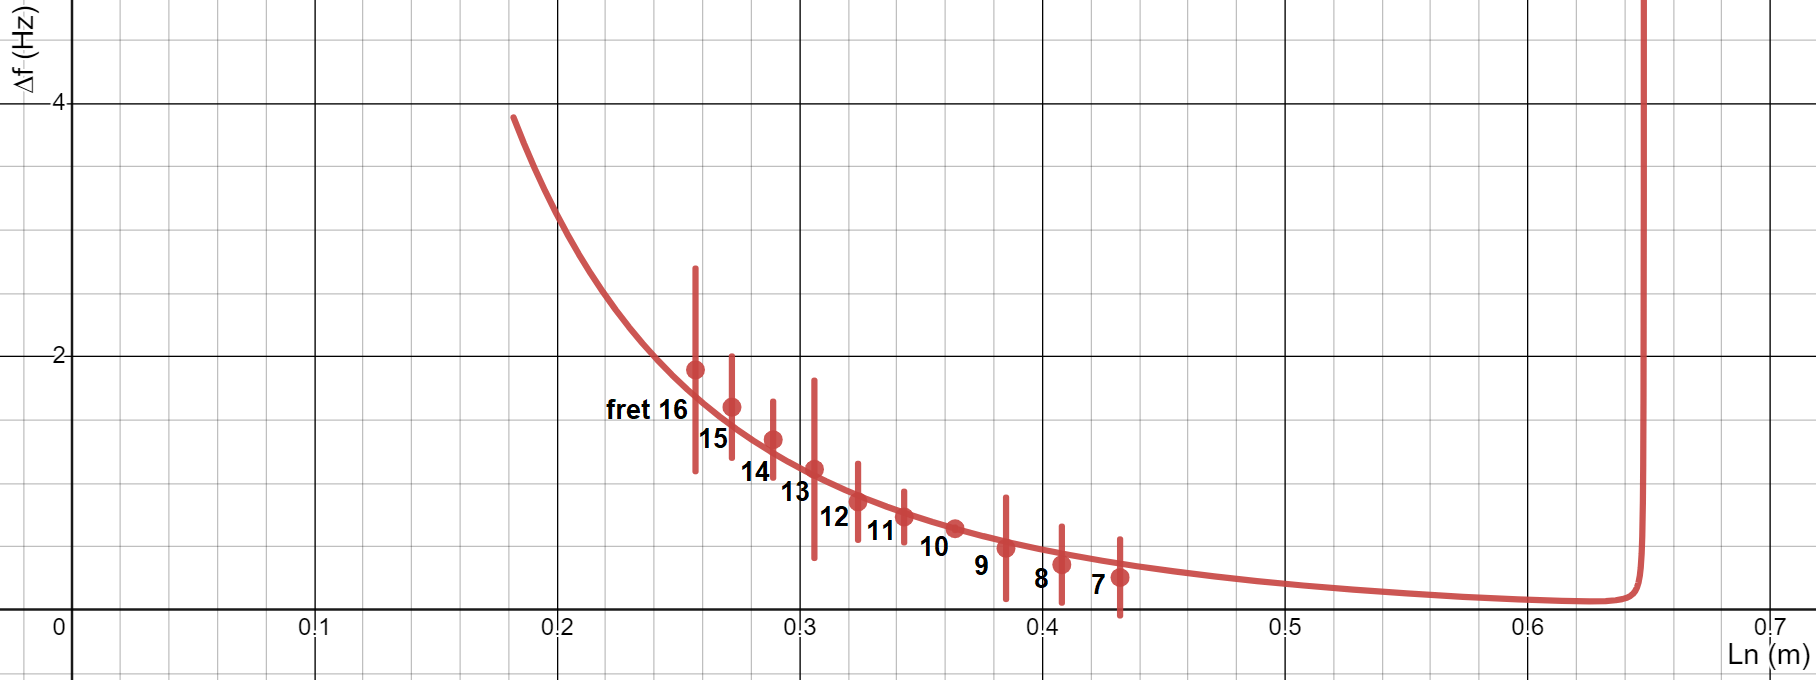
\includegraphics[width = \textwidth]{ee/compare b string.png}
    \caption{Curve for B string with data points and error bars} \label{fig10}
\end{figure}
\begin{figure}[!htb]
    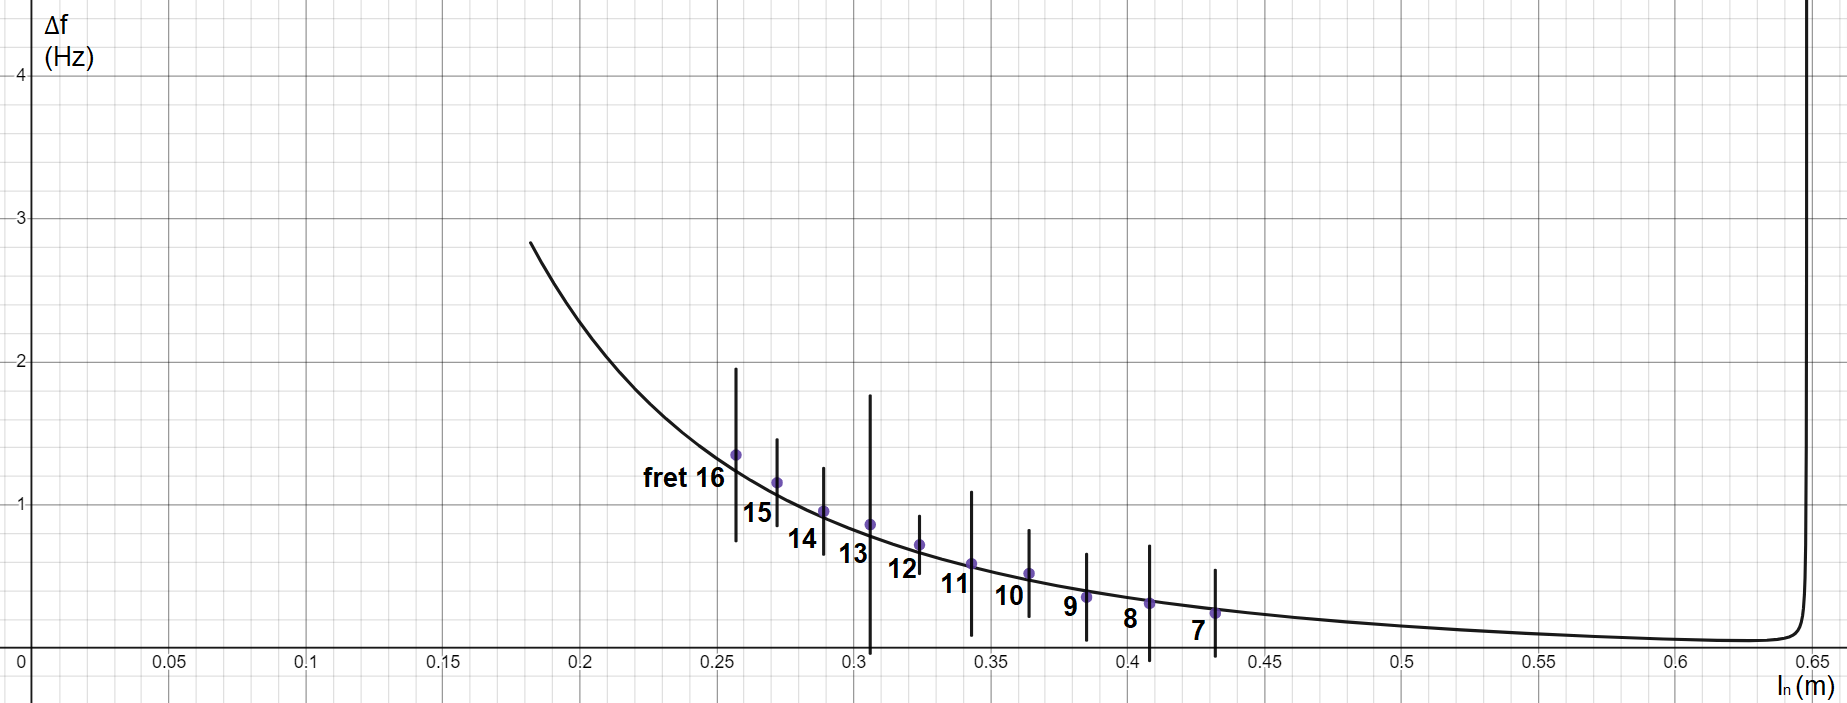
\includegraphics[width = \textwidth]{ee/compare e string.png}
    \caption{Curve for E string with data points and error bars} \label{fig11}
\end{figure}
\begin{figure}[!htb]
    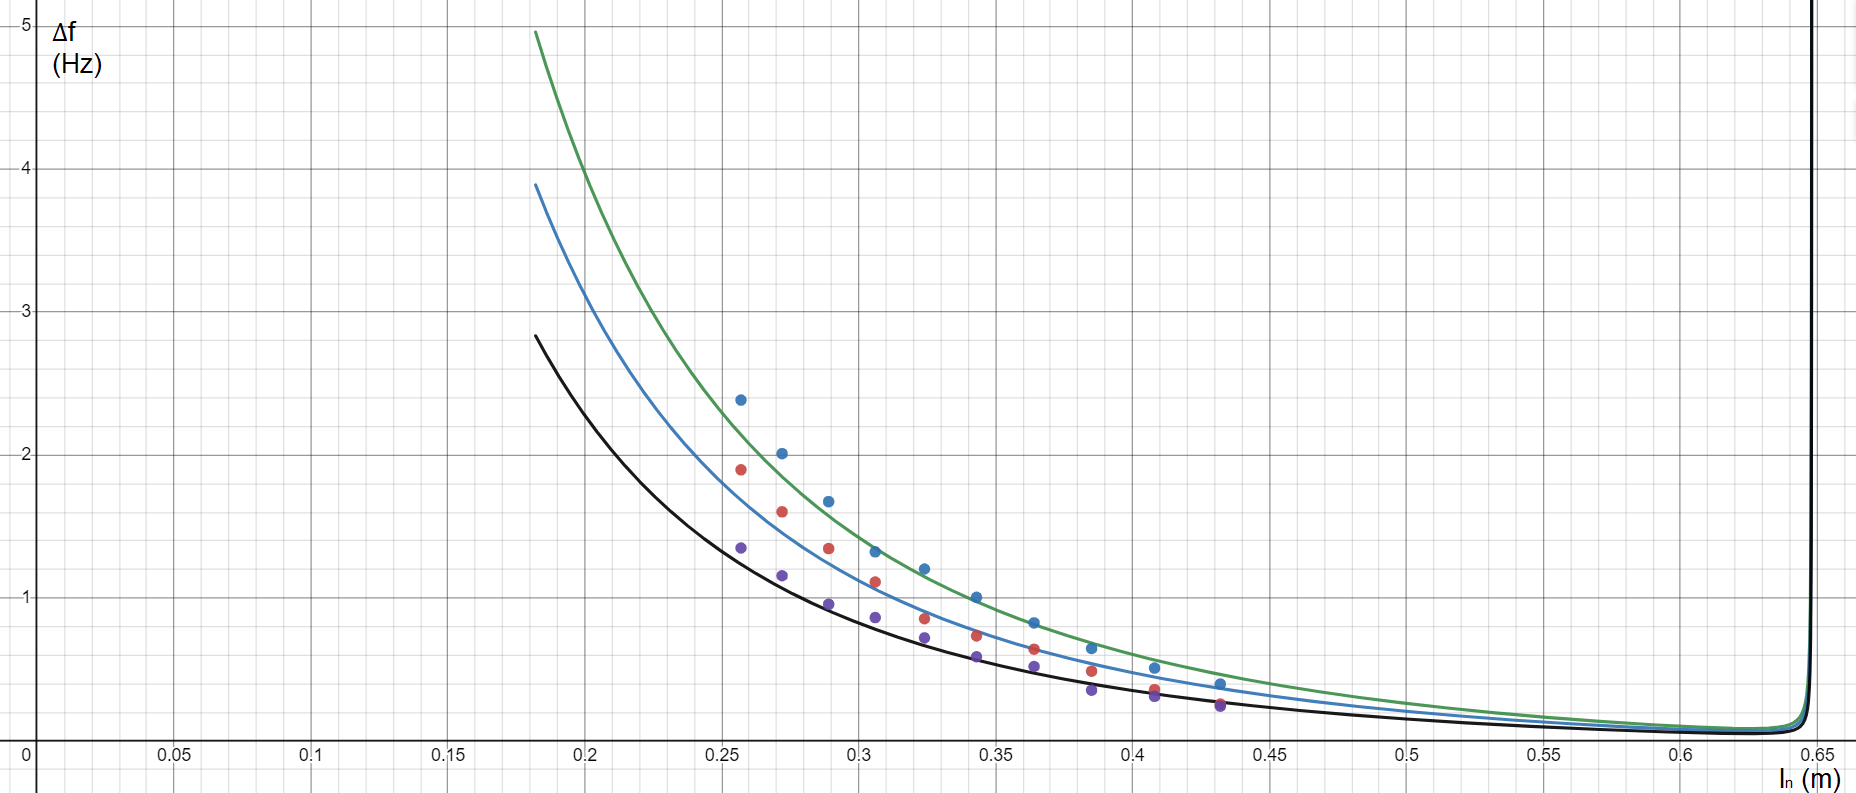
\includegraphics[width = \textwidth]{ee/all 3.png}
    \caption{Curve for all 3 strings with data points} \label{fig12}
\end{figure}
Overall we see that the graphs of B and E strings are successively lower, meaning the intonation deviation on those strings are less, showing that my observation is correct. I believe this is not because of the different string gauges but because the strings have different $f_0$. We can also make some observations; most noticeably, data points for higher frets are slightly higher than predicted by the curve. This is the same trend observed with the original data of the G string, and I believe the cause is the same: the capo not fretting directly down on the string but slightly pushing the string sideways. Also, we can see the error bars generally are smallest for the thickest G string, and biggest for the thinnest E string. This means there is an increase in variance of the frequency for trials at each fret position for thinner strings. This might be because thin strings are more likely to slip a little sideways under the capo when plucked, meaning for the same fret, there will be a slightly different frequency for each pick, although the capo is never moved. It is also noticeable that there is a large error bar at fret 13 and 16 for the B and E strings. Upon closer inspection of the guitar, it seems like the frets at these positions are quite worn down. This might cause the string to slip more under the capo, explaining the large error bar. We also see that the error bars for different strings overlap quite significantly, meaning the results might not be statistically significant, therefore we need to find ways to increase the precision of the measurements to further confirm the relationship. Some improvements I can suggest is to use a stronger capo to minimize slipping or level the guitar frets before carrying out the experiment. We can also try to control the plucking with some mechanism that can consistently deliver the same force to the string to avoid pushing the string sideways too much. 

Guitar players can take this into account when choosing strings. For example, players with a heavier playing style shouldn't choose light gauge strings, because thinner strings with lower resistance are more likely to be pushed sideways rather than directly down on the fret, which will cause intonation shifts.

From the graph of the equation relating $\Delta f$ and $l_n$ we can also evaluate the effects of changing other variables on the shape of the curve. It is impossible to have zero intonation deviation, but I can try to minimize this error. I notice the variable that has the most effect on the graph is $a$, the vertical distance between top of the bridge and the frets. Simply reducing the value of $a$ by around 1.3 mm, bringing it from 3.33 mm down to 2 mm (\SI{2e-3}{m}) is enough to reduce the intonation shift at fret 16 down to around 1.8 Hz (Figure \ref{fig13}), which would be equivalent to $\frac{1.8}{C5-B4}\cdot 100 = \frac{1.8}{523.25-493.88} \cdot 100 \approx 6$ cents, which is almost unnoticeable to the human ear. \cite{loeffler}

\begin{figure}[!h]
    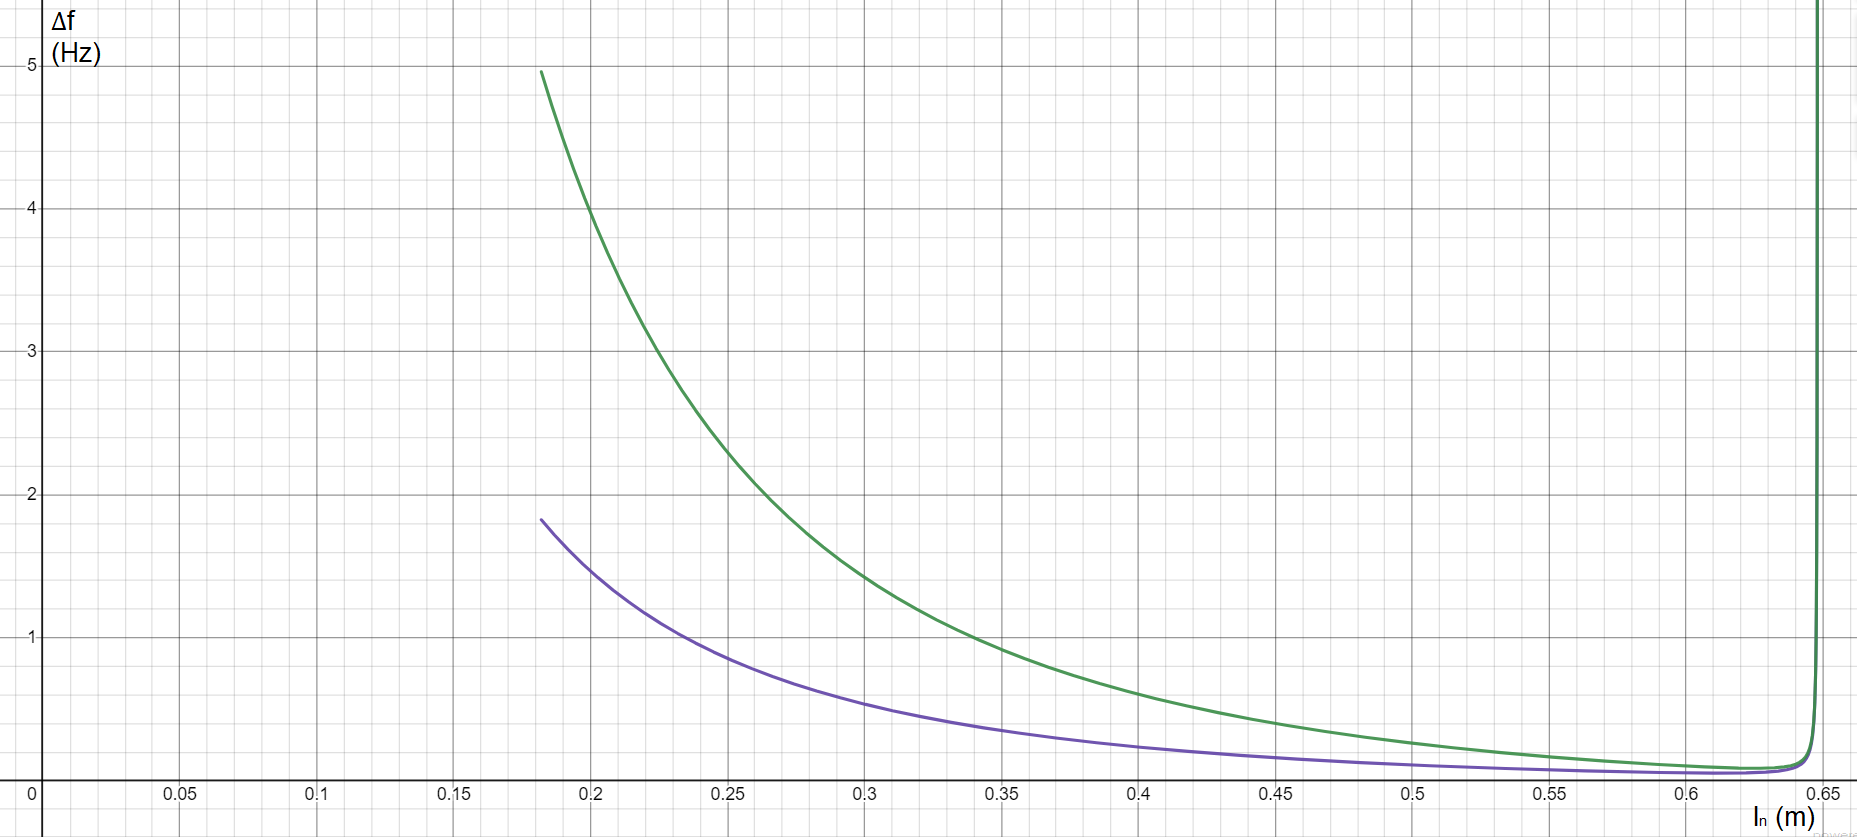
\includegraphics[width = \textwidth]{./ee/compare_graph_a.png}
    \caption{Comparing before (green) and after changing value of $a$ (purple)} \label{fig13}
\end{figure}
So a lower string action would be better for intonation. Guitar manufacturers as well as guitarists can take this into account when setting up their guitars to reduce the intonation error. However, reducing the bridge height too much will cause buzzing of the string, where the string hit against other frets when it is plucked and vibrating. This will reduce the quality of the tone and might even lead to more intonation error. Therefore, a careful trial and error approach is needed when adjusting for a good intonation. \par
Overall from the investigation we see that the intonation of a guitar string is very complicated and affected by a lot of different factors. We cannot eliminate it completely, but there are some things we can do to control it and minimize intonation deviations, such as using thicker strings and having a low action.